\chapter{Simulation-based optimization using gradient methods}
\section{Introduction}
In chapter \ref{chap:sim}, we discussed what the simulator is composed of and how it predicts growth curves for gene knockout experiments. This chapter will handle how
the simulator is used to improve the growth curve predictions of the initial model. In order to test the optimization algorithm, we identified different scenarios which we will 
discuss in the next sections. 
% \section{Model parameter estimation}
% %Simulator based optimization
% \cite{ud2015optimal}
\section{Different scenarios}
Recall from chapter \ref{chap:sim} that the simulator actually consists of a gene regulatory network and a metabolic network. From the point of view of our application,
we are primarily interested in learning the gene regulatory network. The different scenarios are related to what the actual output is and thus what can actually be used
in the optimization problem. In every case the simulator takes as input a knockout experiment, which we will call $\mathbf{exp}$. Additionally we will denote the number of
vertices with $N$ and the number of timesteps $T$.
\subsection{Scenario 1: all gene values at every time step}
In this case the output of the simulator exists of the values of every vertex in the graph at every timestep.
This means the simulator is characterized by, $sim_{1}: \mathbf{exp} \to \mathbb{R}^{N \times T}$. This corrresponds to the case where the GRN (only) contains genes and
where an experiment is performed using microarrays.
\subsection{Scenario 2: the values of a subset of gene at every time step}
Compared to the first scenario, the only difference lies in the fact that instead of using all the vertices in the graph, we can only see a subset of them. This could correspond
to learning a gene regulatory network from microarray experiments for which we cannot see all the concentrations, for instance because there are non-gene vertices.
$sim_{2}: \mathbf{exp} \to \mathbb{R}^{N_{sub} \times T}$, with $N_{sub} \subset N$.
\subsection{Scenario 3: one value per time step obtained by applying some function on gene values}
Instead of the values of the vertices being available at every time step, the values are now aggregated in a function that maps the values to a single value at every time step, $f: \mathbb{R}^{N} \to \mathbb{R}$.
By doing so, the simulator creates a single time series instead of one per vertex in the network. The simulator is the transformed into: $sim_{3}: \mathbf{exp} \to \mathbb{R}^{T}$. 
These functions, that operate as proxies for the FBA, were chosen from typical benchmark problems in optimization theory. In the following descriptions of the different functions, we will denote the output as
$out[t]$, similar to before, $g_i$ denotes the value of the $i$-th vertex and $N$ the amount of vertices in the graph.
\subsubsection{Summation}
\begin{equation}
 y[t] = \sum_{i=1}^N g_i[t]
\end{equation}
\subsubsection{Summations of squared values}
\begin{equation}
 y[t] = \sum_{i=1}^N g_i^2[t]
\end{equation}
\subsubsection{Rosenbrock function}
\begin{equation}
 y[t] = \sum_{i=1}^{N-1}[100(g_{i+1}[t] - g_i^2[t])^2 + (g_i[t] - 1 )^2]
\end{equation}
\subsubsection{Styblinski–Tang function}
\begin{equation}
 y[t] = \sum_{i=1}^n g_i^4[t] - 16g_i^2[t] + 5g_i[t]
\end{equation}
\subsection{Scenario 4: one value per time step, obtained with FBA}
The results of the metabolic genes are fed to the metabolic network by adjusting the corresponding flux rates and the resulting metabolite fluxes are passed to the metabolic vertices in the gene regulatory network
as described in section \ref{sec:fba}.
% \cite{varma1994stoichiometric}
% \cite{hoffner2013reliable}
% \cite{gomez2014dfbalab}
% \cite{chandrasekaran2010probabilistic}
% \cite{colijn2009interpreting}
\section{Parameters}\label{sec:params}
There are two different sets of parameters that can be optimized, those related to the GRN and those related to the metabolic network. In scenarios 1 to 3, only the GRN parameters are to be optimized, in scenario 4 
both sets. A short description of these is provided in the next sections.
\subsection{GRN parameters}
Previously, we already discussed that the simulator's gene regulatory network has parameters associated with their vertices and edges.
Given equation \ref{eq:gene_update}, we can define a matrix of parameters related to the adjacency matrix of the underlying network:
\begin{equation}
\mathbf{W} = \begin{bmatrix} 
\theta_{e,(1,1)} &\cdots & \theta_{e,(1,N)}\\
\vdots & \ddots & \vdots \\
\theta_{e(N,1} & \cdots & \theta_{e,(N,N)} 
      \end{bmatrix}
\end{equation}
and

\begin{equation}
 \boldsymbol{\theta_v} = \begin{bmatrix}
     \theta_{v,1} \\
      \vdots \\
      \theta_{v,N} 
     \end{bmatrix}
\end{equation}

Where $\theta_{e,(i,j)}$ is non-zero if there is a directed edge from vertex $i$ to $j$ and the value being the influence that vertex $i$ has on $j$ and $\theta_{v,i}$ is a constant term indicating the behaviour on the level of a vertex $i$ 
when there is no interaction (i.e. the incoming nodes have level 0) cfr. equation \ref{eq:gene_update}. This gives us the following vector of parameters:
\begin{equation}
 \mathbf{\theta} = \begin{bmatrix}
                     \theta_{e,(1,1)} \\
                     \vdots \\
                     \theta_{e,(N,N)} \\
                     \theta_{v,1} \\
                     \vdots \\
                     \theta_{v,N}
                    \end{bmatrix}
% 
\end{equation}
\subsection{Metabolic network parameters}
Additionally we parametrized how the gene regulatory network interacts with the metabolic network similar by adjusting the fluxes 
by incorporating gene expression levels as in \cite{chandrasekaran2010probabilistic}.
As the gene regulatory network generates continuous values, we apply
a logistic function to map these to the interval $[0,1]$. 
In the equation of the logistic curve 
\begin{equation}
 f(x) = \frac{L}{1+e^{-k(x-x0)}}
\end{equation}
To allow for the correct range, we keep $L$ fixed to 1. This however leaves other parameters that need to be set: $k$ and $x0$, so for every gene that influences the metabolic
network there are 2 additional parameters. The metabolic network contains a total of 904 genes\footnote{In the metabolic model iMM904}, whereas the gene regulatory
network for diauxic shift contains 333 genes. Taking the intersection of those two sets yields a total of 146 genes
% \footnote{These are: YBL015W, YLR304C, YJL200C, YAL054C, YLR153C, YOL086C, YMR303C, YMR083W, YBR145W, YCR010C, YCL025C, YBR132C, YMR169C, YOR374W, YER073W, YPL061W, YPR128C, YBR149W, YOR377W, YDR384C, YPL111W, YLR438W, YML042W, YOR125C, YAL038W, YNR001C, YCR005C, YPR001W, YHR051W, YOR100C, YDR256C, YGR088W, YML054C, YJR048W, YJL005W, YOR065W, YML070W, YIR029W, YIR032C, YIR028W, YJR152W, YIR031C, YOR180C, YDL174C, YEL071W, YBR208C, YHL016C, YLR284C, YGR254W, YHR174W, YOR317W, YER015W, YMR246W, YKL060C, YLR377C, YOR388C, YKR009C, YLL043W, YPL262W, YAL062W, YCL040W, YDL022W, YKL152C, YDL021W, YDR098C, YHL032C, YIL155C, YER062C, YFR053C, YGL253W, YHR094C, YMR011W, YDR345C, YHR092C, YHR096C, YDR343C, YDR342C, YER065C, YPR006C, YNL037C, YOR136W, YDL066W, YLR174W, YNL009W, YKL217W, YIL125W, YDR148C, YFL018C, YOR142W, YGR244C, YKL029C, YKL085W, YOL126C, YDL078C, YNL117W, YML120C, YKR097W, YLR044C, YLR134W, YGR087C, YGL248W, YOR360C, YGR240C, YMR205C, YIL107C, YOL136C, YBR196C, YCR012W, YKL127W, YMR105C, YMR006C, YIL160C, YGL205W, YPL147W, YKL188C, YGL062W, YBR218C, YOR347C, YJL166W, YKL148C, YLL041C, YKL141W, YDR178W, YOR184W, YJR095W, YNL202W, YDR536W, YPL057C, YJL052W, YJR009C, YGR192C, YJR019C, YBR117C, YJR066W, YKL203C, YDR050C, YBR126C, YDR074W, YGR019W, YBR006W, YDL210W, YEL021W, YAR035W, YER024W, YJL045W, YNL241C}
The metabolism of yeast is well understood, at least better than the gene regulatory network\cite{NEEDED}. For this reason we primarily parametrize the gene regulatory network and how it interacts with the metabolic network
and leave the metabolic network as is.
\section{Optimization problem}
\subsection{Introduction}
In this section we will discuss several aspects of the optimization problem. This includes the optimization algorithm, adjustments of the standard algorithms, tunable parameters and objective functions.
\subsection{Gradient descent}%http://link.springer.com/chapter/10.1007%2F978-3-642-35289-8_25#page-1
Gradient descent is an optimization method that tries to optimize an objective function by iteratively updating the parameters of its model.
In gradient descent the parameter vector is updated iteratively by calculating the gradient at a certain point and updating the weights in the direction of the negative gradient as this is the direction in which the function is declining. 
In regular gradient descent the calculation of the gradient is done on the whole training set. Given a multi-variable function and parameter vector $\mathbf{x}$
$F(\mathbf{x})$ and if it is defined and differentiable in a certain point $\mathbf{a}$, and given a
certain learning rate $\gamma$  the new point $\mathbf{b}$ is calculated as follows.
\begin{equation} \label{eq:gd}
 \mathbf{b} = \mathbf{a} - \gamma \nabla F(a)
\end{equation}
 \subsection{Stochastic Gradient Descent} 
 Stochastic Gradient Descent(SGD) is a simplification of the Gradient Descent(GD) algorithm. Whereas GD updates the parameter vector by calculating the gradient for all training examples, SGD estimates
 the gradient based on a single randomly picked example, resulting in a noisier approximation of the gradient.
 \subsection{Objective Function}\label{section:obj}
 Recall that equation \ref{eq:gd} requires us to specify some function $F(\mathbf{x})$ whose value will be minimized. For this work, we employed the Mean Squared Error. As the outputs for the different scenerios
 are not the same, there are some differences in the equations which we will quickly discuss.
 \subsubsection{Scenario 1}
 \begin{equation}
  F_{1}(\mathbf{x}) = \frac{1}{N\cdot T} \sum_{i=1}^N\sum_{t=1}^T(\hat{y}_i[t] - y_i[t])^2
 \end{equation}
 where N is the total amount of values, which is the amount of genes multiplied with the amount of time steps, $i$ iterates
 over all these values, $\hat{y}_i$ is the value estimated by the model and $y_i$ is the actual value.
 \subsubsection{Scenario 2}
 \begin{equation}
  F_{2}(\mathbf{x})  = \frac{1}{N_{sub}\cdot T} \sum_{i=1}^{N_{sub}}\sum_{t=1}^T(\hat{y}_i[t] - y_i[t])^2
 \end{equation}
 In this case only a subset $N_{sub} \subset N$ of the vertices is used .
 \subsubsection{Scenarios 3 \& 4}
 \begin{equation}
 F_{3,4}(\mathbf{x}) = \frac{1}{T} \sum_{t=1}^T(\hat{y}[t] - y[t])^2
 \end{equation}
 with $y[t]$ and $\hat{y}[t]$ denote respectively the actual and estimated output of the aggregate function or of the growth curve obtained from FBA at time $t$.
 
\subsection{Gradient of objective function}
In fact, it's not the objective function itself which is needed for the gradient descent algorithm, but rather the gradient of the objective function. If analytical solutions of the derivates
are available, it is better to apply them directly. In some cases however it is not possible to obtain these analytical solutions. In our application this would involve obtaining a closed-form solution
to the optimization problem defined by flux balance analysis, which at the very least is not straightforward. The simplest way to numerically approximate the gradient is the technique of finite differences. 
The approximation consists of obtaining the values for the objective function where a \textit{small} number is added and subtracted for every parameter separately and then dividing the difference of them by two times the \textit{small} number.
This approximation is however highly numerically inefficient as this requires an amount of function evaluations equal to two times the size of the parameter vector.
On the other hand, in simultaneous perturbation stochastic approximation(SPSA)\cite{hazen2009gradient} the gradient is estimated by stochastically choosing a direction
in which to perturb the operating point to calculate a finite difference gradient. 

\begin{equation}
 \hat{\nabla f(c)}[d] = \frac{f(x_k + \delta_k\Delta_k[d]e_d) - f(x_k - \delta_k\Delta_k[d]e_d)}{2\delta_k\Delta_k[d]}
\end{equation}
``where $e_d$ is a $D$-component vector with 1 for the $d$th component and 0 for all other components, $\delta_k$ is a 
scalar that generally shrinks as the number of iterations $k$ increases, and $\Delta_k$ is a random $D$-component perturbation
vector."
This approach only requires 2 evaluations of $f$ to calculate a gradient.
%  SPSA \url{http://www.jhuapl.edu/spsa/}
%  SAA \url{https://people.orie.cornell.edu/shane/pubs/SAAGuide.pdf} sample average approximation, \url{http://www.stat.columbia.edu/~liam/teaching/compstat-spr15/lauren-notes.pdf}

 
\subsection{Learning rates}
It is possible to keep the learning rate $\gamma$ from equation \ref{eq:gd} fixed throughout the different iterations, however previous studies have shown that improved convergence can be obtained by allowing
$\gamma$ to be altered in subsequent iterations \cite{jacobs1988increased}. These techniques are however still sensitive to the initial choice of the learning rate. A (relatively new) technique called AdaDelta\cite{zeiler2012adadelta}
avoids choosing and having to manually tune a learning rate altogether and good results for this adaptive schemes have been reported. An overview of the revised algorithm is shown in figure \ref{fig:adadelta}.
% \subsection{AdaGrad}
% \cite{duchi2011adaptive}
\begin{figure}	
    \centering
    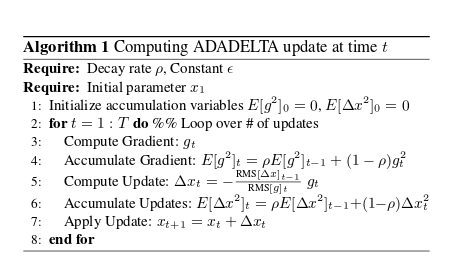
\includegraphics[width=0.4\textwidth]{images/ada_delta.png}
    \caption{ An overview of the AdaDelta algorithm. }
    \label{fig:adadelta}
\end{figure}
\subsection{Stopping mechanism}
To avoid overfitting an early stopping mechanism is applied on a whithheld validation set\footnote{Training set, validation set and test set are divided 
in respectively 60\%-20\%-60\%.}. If the performance does not improve for a preset amount of iterations, the algorithm is terminated and returns the best parameter vector before those 50 iterations.
Apart from that strategy, some other methods were also implemented in order to save on computation time:
\begin{enumerate}
 \item The maximum amount of epochs is parametrized. When the optimizer reaches this amount, it stops and returns the currently optimal value.
 \item We also calculate the errors between epochs. When the average absolute error is lower than a preset\footnote{0.00001} tolerance level in the last preset amount of iterations, the optimizer terminates as well and returns the last optimal value.
\end{enumerate}
 \section{Experiments}
 \section{Introduction}
 This section will cover some aspects about the experiments that we perform with the optimization algorithm such as
 how the the datasets were generated or obtained, how we evaluate the results. 
 \subsection{Datasets}
 \subsubsection{Toy datasets}
 We considered two types of networks, complete digraphs\footnote{``A complete digraph is a directed graph in which every pair of distinct vertices is connected by a pair of unique edges (one in each direction).''} and scalefree networks
\footnote{``A network whose degree distribution follows a power law, at least asymptotically. That is, the fraction P(k) of nodes in the network having k connections to other nodes goes for large values of k as 
$ P(k) \sim k^{-\gamma} $ where $\gamma$ is a parameter whose value is typically in the range $2 < \gamma < 3$ \cite{barabasi2004network}, although occasionally it may lie outside these bounds''}. We have opted for this
kind of networks as a lot of real-life networks can be characterized as being scalefree. Examples of such graphs include biological networks such as gene regulatory networks and protein interaction networks, social networks and more \cite{barabasi2009scale}
The parameters related to the vertices and edges are randomly sampled from the normal distribution with mean $0$ and standard deviation $1$. Given this network we then generated a list of all possible knockout experiments(input to the system), and
calculated the outputs with this network and the simulator, adding different levels of noise. These toy datasets were then used for scenarios 1, 2 and 3.
Remark: There has been some discussion about the usage of scalefree networks \cite{LimaMendez09} for biological networks.
 \subsubsection{Eve Growth curves}
 Currently not available.. Needed for scenario 4.
 \subsection{Evaluation}\label{sec:eval} 
To evaluate the output of the parameter estimation algorithm we calculate the mean squared error on a separate testset (see Section \ref{section:obj}) and the Euclidian distance of the optimal
parameter vector to the real parameter vector (see Section \ref{sec:eval}). When using the output of the optimization algorithm as samples we use the kolmogorov-smirnov statistic rather than
the Euclidian distance.
Every set of algorithmic parameters is repeated 10 times with different randomized networks. The length of the time series is kept at 10.

\subsection{ Implementation }
The implementation of the optimization algorithms can be found at \url{AdaLab/src/optimization} of the evaluation code in \url{adalab/src/executables}. Additionally, 
some parts of the implementations are exposed to R. These exposed classes and methods are found in the file \url{AdaLab/src/R_interface_optimization.cpp}.
\subsection{Discussion}
The results showed non-sparse networks and thresholding the learned values did not show a correlation with the true edges. As this is highly unlikely, we changed the approach in order to learn more sparse structures and
obtain a distribution over networks.
